\documentclass[10pt]{article}

% Cargo los archivos con el formato
%% Para buscar documentacion de paquetes: http://texdoc.net/

% Formato de pagina{{{
% Fuente
\usepackage[]{times}

% Pagina
\usepackage[]{geometry} %Para definir donde se ubica el texto
\geometry{a4paper,textwidth={17cm},textheight={23cm},left={2cm},top={2.5cm},}

% Encabezado y Pie de pagina
\usepackage[]{fancyhdr}
\pagestyle{fancy}
\renewcommand{\headrulewidth}{0pt} % para que no haya linea decorativa en el header.

% Columnas
\usepackage[]{multicol} %Para poder usar columnas
\setlength{\columnsep}{1cm} %Separacion entre columnas de 1 cm

% Para definir afiliaciones de autores
\usepackage[]{authblk} 

% Formato de fecha
\usepackage{datetime2}
\DTMsetstyle{iso}

% Para poder poner numero total de paginas en pie de pagina
%\usepackage{lastpage}
\usepackage[pagecontinue=false]{pageslts}

% Secciones{{{
\usepackage[]{titlesec} % Da formato a secciones
%% Seccion
%\titleformat{\section}
%{\normalfont\large\bfseries\MakeUppercase}{\thesection.}{.3em}{}
%\titlespacing*{\section}{0cm}{0.25cm}{0.15cm}

%% Subseccion
%\titleformat{\subsection}
%{\normalfont\large\bfseries}{\thesubsection.}{.3em}{}
%\titlespacing*{\subsection}{.15cm}{0.2cm}{0.1cm}

%%Subsubseccion
%\titleformat{\subsubsection}
%{\normalfont\normalsize\bfseries}{\thesubsubsection.}{.3em}{}
%\titlespacing*{\subsubsection}{0.25cm}{0.15cm}{0.05cm}

%\titleformat{\caption}
%{\normalfont\normalsize\bfseries}{\thesubsubsection.}{.3em}{}
%\titlespacing*{\subsubsection}{0.25cm}{0.15cm}{0.05cm}
%}}}

%}}}

% Figuras y tablas{{{
\usepackage[]{graphicx}
\usepackage[space]{grffile} %Por si nombre de archivo tiene espacios

\usepackage[]{float} %Para poder usar [H] para poner fig correctamente en 2 columnas

\graphicspath{{img/}} %Defino carpeta para figuras

% Tablas
% Algunas opciones
%\usepackage{array}
%\usepackage{tabulary}
%\usepackage{tabularx}
% El que mejor resultado da para 2 columnas
\usepackage{tabu}


% Captions(Epigrafes)
% Para que la fuente de un epigrafe no tenga el mismo tamaño que el cuerpo del texto, tambien le indico donde va a estar para cada caso
\usepackage[font=small,skip=0.3cm,tableposition=top,figureposition=bottom,justification=centering]{caption}

%}}}

% Listas{{{

% Para listas
% Para que las listas numeradas acepten opciones
\usepackage[]{enumerate} 

%}}}

% Ecuaciones{{{
%  Mas opciones de formato para ecuaciones
\usepackage[]{amsmath}
\usepackage[]{amsfonts}%Requerido por amsmath

%}}}

% Bibliografía{{{
\usepackage[sorting=none,backend=biber]{biblatex}
\addbibresource{bibliografia.bib}
%}}}

% Otros{{{
\usepackage[hidelinks]{hyperref} % Para usar hipervinculos
\usepackage[]{verbatim} % Para poder comentar por bloques
\usepackage[]{lipsum} % Para rellenar con texto

%}}}

% Anexo{{{
%Para poder utilizar anexos
%\usepackage[toc,page]{appendix}

%Fix para appendix y hyperref con español%{{{
%\makeatletter
%\let\oriAlph\Alph
%\let\orialph\alph
%\renewcommand{\@resets@pp}{\par
%\@ppsavesec
%\stepcounter{@pps}
%\setcounter{section}{0}
%\if@chapter@pp
%\setcounter{chapter}{0}
%\renewcommand\@chapapp{\appendixname}
%\renewcommand\thechapter{\@Alph\c@chapter}
%\else
%\setcounter{subsection}{0}
%\renewcommand\thesection{\@Alph\c@section}
%\fi
%\if@pphyper
%\if@chapter@pp
%\renewcommand{\theHchapter}{\theH@pps.\oriAlph{chapter}}
%\else
%\renewcommand{\theHsection}{\theH@pps.\oriAlph{section}}
%\fi
%\def\Hy@chapapp{appendix}
%\fi
%\restoreapp
%}
%\makeatother}}}

%}}}

% Comandos propios{{{

% Para que el titulo y autor tengan el formato que corresponde
\newcommand{\titulo}[1]{\title{\Large\bfseries\MakeUppercase{#1}} }
\newcommand{\autor}[1]{\author{\bfseries\MakeUppercase{#1}} }

% Para que los mail tengan hipervinculos
\newcommand{\emailttt}[1]{\texttt{\href{mailto:#1}{#1}} }
\newcommand{\email}[1]{\href{mailto:#1}{#1}}

% Para utilizar variables para la materia y fecha
\newcommand{\materia}[1]{\newcommand{\materiavar}{#1}}
\newcommand{\Rheader}[1]{\newcommand{\fechavar}{#1}}
\fancypagestyle{titlestyle}{
    \fancyhead[R]{\fechavar}
    \fancyhead[L]{\materiavar}
}

% Para insertar titulo
\newcommand{\institulo}[0]{ \
    \noindent \
    {\begin{minipage}{\textwidth} \
	    \centering \
	    \maketitle \
	    \thispagestyle{titlestyle} \
    \end{minipage}} \
}


% Contador para numerar secciones correctamente
\newcounter{arabiccount}

\newcommand{\resetnumber}{
    \addtocounter{arabiccount}{1}
    \pagenumbering{Roman} % para resetear numeros
    \pagenumbering{arabic}
}

% Para setear formato de secciones para el documento

\newcommand{\documentformat}{
    % Formato de las secciones
    % Seccion
    \titleformat{\section}
    {\normalfont\large\bfseries\MakeUppercase}{\thesection.}{.3em}{}
    \titlespacing*{\section}{0cm}{0.25cm}{0.15cm}

    % Subseccion
    \titleformat{\subsection}
    {\normalfont\large\bfseries}{\thesubsection.}{.3em}{}
    \titlespacing*{\subsection}{.15cm}{0.2cm}{0.1cm}

    %Subsubseccion
    \titleformat{\subsubsection}
    {\normalfont\normalsize\bfseries}{\thesubsubsection.}{.3em}{}
    \titlespacing*{\subsubsection}{0.25cm}{0.15cm}{0.05cm}

    \titleformat{\caption}
    {\normalfont\normalsize\bfseries}{\thesubsubsection.}{.3em}{}
    \titlespacing*{\subsubsection}{0.25cm}{0.15cm}{0.05cm}

    % Formato de numeros y pie de pagina
    \pagenumbering{arabic}
    \fancyhf{}
    \pagestyle{fancy}
    \fancyfoot[R]{\thepage\ \devar\ \lastpageref*{pagesLTS.arabic.\arabic{arabiccount}} }
}

\newcommand{\docstart}{
    % Formato de la numeracion
    \addtocounter{arabiccount}{1} 
    \documentformat
}

\newcommand{\docstyle}{
    % Formato de la numeracion
    \clearpage
    \resetnumber
    \documentformat
}


% Para formato de secciones de anexos
\newcommand{\appendixformat}[0]{

    % Formato de secciones
    % Seccion
    \renewcommand{\thesection}{\Alph{section}}
    \titleformat{\section}
    {\normalfont\huge\bfseries\MakeUppercase}{\anexovar\ \thesection: }{.3em}{}
    \titlespacing*{\section}{0cm}{0.25cm}{0.15cm}

    % Subseccion
    \titleformat{\subsection}
    {\normalfont\large\bfseries\MakeUppercase}{\thesubsection.}{.3em}{}
    \titlespacing*{\subsection}{0cm}{0.25cm}{0.15cm}

    % Subsubseccion
    \titleformat{\subsubsection}
    {\normalfont\large\bfseries}{\thesubsubsection.}{.3em}{}
    \titlespacing*{\subsubsection}{.15cm}{0.2cm}{0.1cm}



    % Numeracion
    \fancyhf{}
    \pagestyle{fancy}
    \fancyfoot[R]{\anexovar\ \thesection: \thepage\ \devar\ \lastpageref*{pagesLTS.arabic.\arabic{arabiccount}} }
}

\newcommand{\appendixstart}{
    % Numeracion
    \clearpage
    \appendix
    \setcounter{section}{0}
    \resetnumber
    \appendixformat

}

\newcommand{\appendixstyle}{
    % Numeracion
    \clearpage
    \resetnumber
    \appendixformat

}



%}}}


% Selecciono mas opciones de formato seggun el idioma
%% Formato para ingles
% Lenguaje{{{
\usepackage[utf8]{inputenc} % para poder usar tildes y caracteres especiales
\usepackage[english]{babel} % para escribir en español
\usepackage{csquotes}

%}}}

% Otros{{{
% Para uniones en la definición de autores
% paquete authblk
\setlength{\affilsep}{0.5cm}

% Abstract
\renewenvironment{abstract}{
    \noindent\hfill\begin{minipage}{\textwidth}
	Abstract --- \itshape}
    {\par\end{minipage}\vspace{1cm}}

    % Para union de numeros de pagina
    \newcommand{\devar}{of}

    % Para nombres de anexos
    \newcommand{\anexovar}{Appendix}

%}}}
 % ingles
% Formato para español
% Lenguaje{{{
\usepackage[utf8]{inputenc} % para poder usar tildes y caracteres especiales
\usepackage[spanish,es-tabla]{babel} % para escribir en español
\usepackage{csquotes}
\usepackage{listings}
\usepackage{amsmath}
\usepackage[T1]{fontenc}

%}}}

% Otros{{{
% Para uniones en la definición de autores
% paquete authblk
\renewcommand\Authsep{, }
\renewcommand\Authand{ y }
\renewcommand\Authands{ y }
\setlength{\affilsep}{0.5cm}

% Abstract
\renewenvironment{abstract}{
    \noindent\hfill\begin{minipage}{\textwidth}
	Resumen --- \itshape}
    {\par\end{minipage}\vspace{1cm}}

    % Para union de numeros de pagina
    \newcommand{\devar}{de}

    % Para nombres de anexos
    \newcommand{\anexovar}{Anexo}

%}}}
 % español


%%% Opciones Generales del documento%{{{
\materia{Procesamiento Digital de Señales}
\Rheader{\today, Argentina}

\titulo{Titulo del TP}

\author[1]{Alumno 1} 
\author[2]{Alumno 2}
\author[3]{Alumno 3}

\affil[1]{Universidad Nacional de Tres de Febrero\protect\\ \email{mail1@gmail.com}}
\affil[2]{Universidad Nacional de Tres de Febrero\protect\\ \email{mail2@gmail.com}}
\affil[3]{Universidad Nacional de Tres de Febrero\protect\\ \email{mail3@gmail.com}}
\date{} %Dejar blanco para que no aparezca la fecha en el titulo

%}}}

% INICIO DEL DOCUMENTO%{{{

\addbibresource{bibliografia.bib}

\begin{document}
\lstset{language=Python}
\lstset{frame=lines}
%\lstset{caption={Insert code directly in your document}}
\lstset{label={lst:code_direct}}
\lstset{basicstyle=\footnotesize}

% Titulo y abstract %{{{
\institulo % Comando propio, inserta el titulo

\docstart % Comando propio, setea el formato de documento
\begin{abstract}
Lorem ipsum dolor sit amet, consectetur adipiscing elit. In ultrices ut ante vehicula venenatis. Aenean non commodo dui. Ut lacus diam, posuere nec scelerisque eget, lacinia eu massa. Fusce finibus nibh at consequat sagittis. Curabitur rutrum fermentum odio nec facilisis. Quisque dapibus egestas vehicula. Nunc ac velit vel nisl condimentum euismod ac vitae dolor. Ut gravida tristique enim a sodales. Donec mollis consequat ipsum, at egestas purus tempus id. Sed elementum lectus id augue rutrum tempor. Nulla facilisi. Sed ornare magna accumsan, tempor quam ac, accumsan nulla. Suspendisse sit amet risus sed nisi viverra volutpat. Donec vitae lorem eu erat condimentum commodo quis non sapien. Vivamus mollis neque id nulla efficitur bibendum.
\end{abstract}


%}}}

% Comienzo de doble columnas
\begin{multicols*}{2} % Pongo el '*' para que no terminen parejas

    \section{Introducción}
Lorem ipsum dolor sit amet, consectetur adipiscing elit. Quisque at nisl sed quam fermentum ultrices id nec turpis. Donec et est nulla. Donec porttitor, mi vel aliquet fringilla, neque lacus aliquam ligula, non laoreet felis purus at ipsum. Quisque at gravida tortor. Donec id nisi ligula. Vivamus ornare quis nibh ut bibendum. Mauris pulvinar risus risus, eu luctus ligula tincidunt vitae. Nunc sit amet placerat nulla, id laoreet metus. Sed euismod elementum pulvinar. Quisque et velit porttitor, volutpat magna vitae, finibus nulla. Sed bibendum cursus dolor eget bibendum. Duis a est sed urna viverra fermentum.

Aliquam volutpat, risus sit amet bibendum semper, erat velit congue mi, eu interdum dolor sem id magna. Fusce sed ipsum ac lorem lacinia ultricies id at justo. Morbi vehicula luctus lacus, eu scelerisque dui congue quis. In ac quam maximus, accumsan nibh vitae, pharetra quam. Quisque euismod justo mi. Ut faucibus ullamcorper lacus non congue. Vestibulum porta erat volutpat, auctor lorem in, commodo nisi. Maecenas tincidunt arcu id odio ullamcorper tristique.


    \section{Marco teórico}

Lorem ipsum dolor sit amet, consectetur adipiscing elit. Quisque at nisl sed quam fermentum ultrices id nec turpis. Donec et est nulla. Donec porttitor, mi vel aliquet fringilla, neque lacus aliquam ligula, non laoreet felis purus at ipsum. Quisque at gravida tortor. Donec id nisi ligula. Vivamus ornare quis nibh ut bibendum. Mauris pulvinar risus risus, eu luctus ligula tincidunt vitae. Nunc sit amet placerat nulla, id laoreet metus. Sed euismod elementum pulvinar. Quisque et velit porttitor, volutpat magna vitae, finibus nulla. Sed bibendum cursus dolor eget bibendum. Duis a est sed urna viverra fermentum.

Aliquam volutpat, risus sit amet bibendum semper, erat velit congue mi, eu interdum dolor sem id magna. Fusce sed ipsum ac lorem lacinia ultricies id at justo. Morbi vehicula luctus lacus, eu scelerisque dui congue quis. In ac quam maximus, accumsan nibh vitae, pharetra quam. Quisque euismod justo mi. Ut faucibus ullamcorper lacus non congue. Vestibulum porta erat volutpat, auctor lorem in, commodo nisi. Maecenas tincidunt arcu id odio ullamcorper tristique.
    
    \section{Procedimiento}
Lorem ipsum dolor sit amet, consectetur adipiscing elit. Quisque at nisl sed quam fermentum ultrices id nec turpis. Donec et est nulla. Donec porttitor, mi vel aliquet fringilla, neque lacus aliquam ligula, non laoreet felis purus at ipsum. Quisque at gravida tortor. Donec id nisi ligula. Vivamus ornare quis nibh ut bibendum. Mauris pulvinar risus risus, eu luctus ligula tincidunt vitae. Nunc sit amet placerat nulla, id laoreet metus. Sed euismod elementum pulvinar. Quisque et velit porttitor, volutpat magna vitae, finibus nulla. Sed bibendum cursus dolor eget bibendum. Duis a est sed urna viverra fermentum.

Aliquam volutpat, risus sit amet bibendum semper, erat velit congue mi, eu interdum dolor sem id magna. Fusce sed ipsum ac lorem lacinia ultricies id at justo. Morbi vehicula luctus lacus, eu scelerisque dui congue quis. In ac quam maximus, accumsan nibh vitae, pharetra quam. Quisque euismod justo mi. Ut faucibus ullamcorper lacus non congue. Vestibulum porta erat volutpat, auctor lorem in, commodo nisi. Maecenas tincidunt arcu id odio ullamcorper tristique.(\ref{señalfiltrada}):

\begin{equation} \label{señalfiltrada}
    y[n] = s[n]-0.9 s[n-1]
\end{equation}

donde $y[n]$ es la señal luego de aplicar el filtro y $s[n]$ es la señal original.

Lorem ipsum dolor sit amet, consectetur adipiscing elit. Quisque at nisl sed quam fermentum ultrices id nec turpis. Donec et est nulla. Donec porttitor, mi vel aliquet fringilla, neque lacus aliquam ligula, non laoreet felis purus at ipsum. Quisque at gravida tortor. Donec id nisi ligula. Vivamus ornare quis nibh ut bibendum. Mauris pulvinar risus risus, eu luctus ligula tincidunt vitae. Nunc sit amet placerat nulla, id laoreet metus. Sed euismod elementum pulvinar. Quisque et velit porttitor, volutpat magna vitae, finibus nulla. Sed bibendum cursus dolor eget bibendum. Duis a est sed urna viverra fermentum.

Aliquam volutpat, risus sit amet bibendum semper, erat velit congue mi, eu interdum dolor sem id magna. Fusce sed ipsum ac lorem lacinia ultricies id at justo. Morbi vehicula luctus lacus, eu scelerisque dui congue quis. In ac quam maximus, accumsan nibh vitae, pharetra quam. Quisque euismod justo mi. Ut faucibus ullamcorper lacus non congue. Vestibulum porta erat volutpat, auctor lorem in, commodo nisi. Maecenas tincidunt arcu id odio ullamcorper tristique. Figura \ref{fig:hamming} \cite{rabinerlargo}.

\begin{figure}[H]
    \centering
    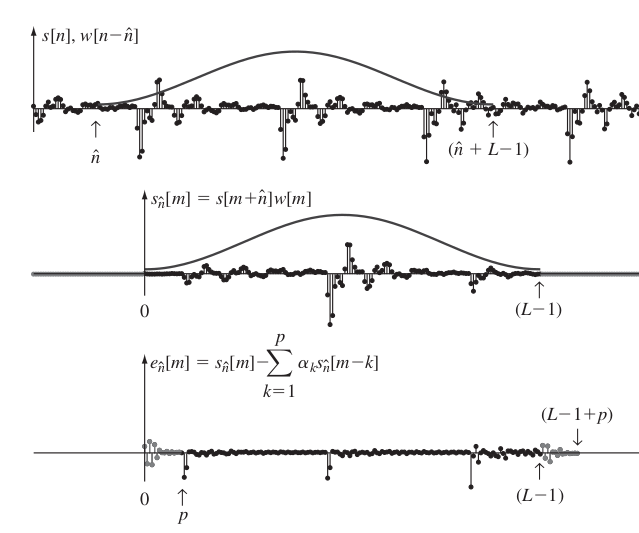
\includegraphics[scale=0.3]{img/hamming.png}
    \caption{Efecto de la ventana de Hamming en los extremos de un frame.}
    \label{fig:hamming}
\end{figure}



    
    \section{Resultados y análisis}

Lorem ipsum dolor sit amet, consectetur adipiscing elit. Quisque at nisl sed quam fermentum ultrices id nec turpis. Donec et est nulla. Donec porttitor, mi vel aliquet fringilla, neque lacus aliquam ligula, non laoreet felis purus at ipsum. Quisque at gravida tortor. Donec id nisi ligula. Vivamus ornare quis nibh ut bibendum. Mauris pulvinar risus risus, eu luctus ligula tincidunt vitae. Nunc sit amet placerat nulla, id laoreet metus. Sed euismod elementum pulvinar. Quisque et velit porttitor, volutpat magna vitae, finibus nulla. Sed bibendum cursus dolor eget bibendum. Duis a est sed urna viverra fermentum.

Aliquam volutpat, risus sit amet bibendum semper, erat velit congue mi, eu interdum dolor sem id magna. Fusce sed ipsum ac lorem lacinia ultricies id at justo. Morbi vehicula luctus lacus, eu scelerisque dui congue quis. In ac quam maximus, accumsan nibh vitae, pharetra quam. Quisque euismod justo mi. Ut faucibus ullamcorper lacus non congue. Vestibulum porta erat volutpat, auctor lorem in, commodo nisi. Maecenas tincidunt arcu id odio ullamcorper tristique.
    
    \section{Conclusiones}
Lorem ipsum dolor sit amet, consectetur adipiscing elit. Quisque at nisl sed quam fermentum ultrices id nec turpis. Donec et est nulla. Donec porttitor, mi vel aliquet fringilla, neque lacus aliquam ligula, non laoreet felis purus at ipsum. Quisque at gravida tortor. Donec id nisi ligula. Vivamus ornare quis nibh ut bibendum. Mauris pulvinar risus risus, eu luctus ligula tincidunt vitae. Nunc sit amet placerat nulla, id laoreet metus. Sed euismod elementum pulvinar. Quisque et velit porttitor, volutpat magna vitae, finibus nulla. Sed bibendum cursus dolor eget bibendum. Duis a est sed urna viverra fermentum.

Aliquam volutpat, risus sit amet bibendum semper, erat velit congue mi, eu interdum dolor sem id magna. Fusce sed ipsum ac lorem lacinia ultricies id at justo. Morbi vehicula luctus lacus, eu scelerisque dui congue quis. In ac quam maximus, accumsan nibh vitae, pharetra quam. Quisque euismod justo mi. Ut faucibus ullamcorper lacus non congue. Vestibulum porta erat volutpat, auctor lorem in, commodo nisi. Maecenas tincidunt arcu id odio ullamcorper tristique.

    \printbibliography

\end{multicols*}


%\appendixstart

%\section{Figura y tabla de ejemplo}
%\begin{multicols*}{2}

%\begin{figure}[H]
    \centering
    \includegraphics[width=\linewidth]{figura.png}
    \caption{Figura de ejemplo.}
    \label{fig:ejemplo}
\end{figure}

\begin{table}[H]
    \centering
    \caption{Tabla de ejemplo}
    \label{tab:ejemplo}
    \begin{tabu} to \linewidth{|L|L|}
	\hline
	Columna1 & Columna2 &
	\hline
	Ejemplo & Ejemplo &
	\hline
    \end{tabu}
\end{table}


%\end{multicols*}

\end{document}

%}}}
